\documentclass[../main.tex]{subfiles}

\begin{document}
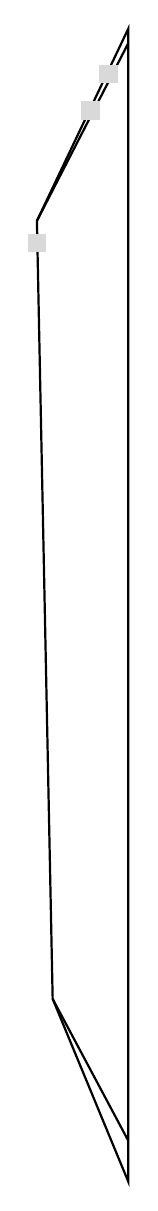
\begin{tikzpicture}[
    scale=0.08,
    sensor/.style={draw=red!60, fill=red!5},
    diffuser/.style={thick,fill=gray!30},
    every path/.style={thick}
]


\coordinate (S1) at (66,25);
\coordinate (S2) at (66,208);
\coordinate (S3) at (51.5,177.5);
\coordinate (S4) at (54, 54);

% For pespective
\coordinate (P1) at (66,31.5);
\coordinate (P2) at (66,205.7);

% Diffusers
%\coordinate (DT) at (62.9,200.8);

\draw (S1) -- (S2) -- (S3) -- (S4) -- cycle;
\draw (P1) -- (S4);
\draw (P2) -- (S3);

\node[diffuser] (DT) at (62.9,200.8) {};
\node[diffuser] (DM) at (60,195) {};
\node[diffuser] (DB) at (51.5,174) {};

\end{tikzpicture}
\end{document}
